\documentclass[11pt]{article}
\usepackage{tikz}
\usetikzlibrary{trees}
\usepackage{amsfonts}
\usepackage{amsmath}
\usepackage{verbatim}
\setlength\parindent{0pt}
\begin{document}
\title{{ModLang}\\
{Good Practices}}
\author{Zachary Kieda (zkieda@andrew.cmu.edu)}
\date{\today}
\maketitle

Note: This article is written for some future implementation of modlang. Currently, we just have the general phases completed to the spec. In a future version, we hope that the initialization could be made easier. Possibly we will make a tailor-made language built for the ModLang functionality that supports high level composition of modules in the manner expressed below. \\

Currently, we just replace constuctors with autowired initialization -- we link items together rather than explicit constructor passing.

\begin{comment}
Idea : we could have modules be used for a new type of composition that's highly expressive.

Example: 

fn =  + : has 
   (_ * 3) (_ * 2)
 end : (_ / 10, _ mod 10)

fn(35) 
  = 
    + : has
      (_ * 3) (_ * 2)
    end : (3, 5)
  = 
    + : has
      9 10
    end
  = 19
  
We could then use this as a high-level composition of classes and their contents, as well as a broader version of function composition.
\end{comment}

\begin{section}{Semantics}
Here, we will go over the semantics of module initialization that we use for the CrowdSimulation project. As we know, ModLang will generate a tree structure of modules. But what about the order and selection of dependency injection, and the initialization techniques that are used. Figure 1 displays an example tree that we will use to display the semantics.

\begin{center}
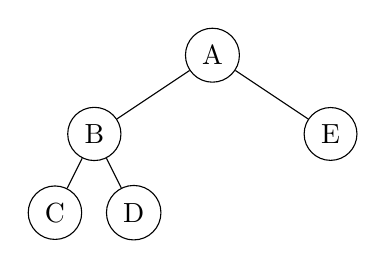
\begin{tikzpicture}[level distance=1.0cm,
level 1/.style={sibling distance=3.0cm},
level 2/.style={sibling distance=1cm}]
\tikzstyle{every node}=[circle,draw]

\node (Root) {A}
    child {
    node {B} 
    child { node {C} }
    child { node {D} }
}
child {
    node {E}
};

\end{tikzpicture}\\
Figure 1 -- An example ModLang class tree
\end{center}

\begin{subsection}{Phase 1 : Linking}
In the first phase, after the class tree is generated, we link modules together -- we insert resources that have the \verb|@AutoWired| annotation. We find resources in the specified manner -- we first run a BFS from the current node to child nodes find the module. Then, we perform a BFS from the current node to the parent node if we did not find the module in the children.\\

Suppose we wanted to inject module D into module A. The priority of modules we use is B-E-C-D. In the case the module is not found in the children, like if we were injecting module E into module B, the priority we would use is C-D-A-E.\\

\textbf{Note:} during this period we allow a single module to accept an arbitrary number of modules by using the syntax \\\verb|@AutoWired java.util.Collection<T extends SubModule>| where \verb|T| is the type of the submodule the client wants to capture. This is processed in this stage.
\end{subsection}

\begin{subsection}{Phase 2 : Initialization}
This is the stage that initializes all of the objects in the hierarchy by running its internal \verb|init()| method. This process must be manually started by the client by calling \verb|init(null)| at the root of the tree. We this because there may be external initialization parameters that the client may want to insert before initialization. A typical example is if the module tree uses \verb|String[] args| as a parameter. In the example below we inject \verb|String[] args| into \verb|ArgsListenerModule|.

\begin{verbatim}
MyModule root = 
    ConstructModule.build(new File("mymodule.mod"));

Optional<ArgsListenerModule> arg = 
    root.getModuleByClass(ArgsListenerModule.class);
    
if(arg.isPresent()){
    arg.get().init(args);
}

root.init(null);
\end{verbatim}

Intuitively, initialization is performed by initializing dependencies before initializing the parent. For example, the initialization strategy we would use from Figure 1 is C-D-B-E-A. Note that the root is initialized last, and children are initialized from left to right. This resembles the composition you would see in plain java code, seen below
\begin{verbatim}
//Same initialization order
//Represents Fig. 1
new A(new B(new C(), new D()), new E());
\end{verbatim}\\

After this phase is complete, we consider all of the modules in this tree to be ``complete" in its initialization, and ready to run as a system. This initialization of a tree is akin to the initialization of a java class.
\end{subsection}

\begin{subsection}{Phase 3 : Listeners}
Listener processing occurs immediately after initialization has completed. A module has the option of listening for new modules that are added to the module tree. Initially, we process the modules that are inside of the same linking unit.\\

In the same unit, we follow a two step process. First, we collect the list of listeners is in the same order used in Section 1.2 (C-D-B-E-A). Then, we process the applicable listeners for each module in the same manner. This is done for two reasons, 1) we want to apply the dependent listeners before applying the parent listeners; the parent may expect some invariant of the child, 2) we process the modules bottom-up since we want the dependent modules processed before the parent.\\ 

Finally, after all of the local listeners have been resolved, we process modules that are directly added to this tree. We only check the root of the module added to this tree, and not children of the root.
\end{subsection}
\end{section}

\begin{section}{Stateless Modules}
In stateless modules, we want to treat each module as if it were a function. By stateless, we mean that the module should not carry any state \emph{after} its external initialization. All initialization should be done by stateless modules. During initialization, state-based modules should only have their initial state set up by other stateless modules. \\

For example, we may want to inject the \verb|String[] args| to a module that processes the command line arguments. This is done after linking and before initialization as described in Section 1.2. Then, the module should only be a supplier for a representation of the command line arguments and not change its state. Stateless modules should be used to initialize state-based modules. Alternatively, stateless modules should be used by state holding modules during the runtime as supporting functions.\\

By convention, stateless modules should be thought of like function composition with respect to the tree structure of the module tree. For example, suppose \verb|B|, \verb|C|, and \verb|D| are stateless from Figure 1. Then the module \verb|B| represents a function that takes \verb|C| and \verb|D| as inputs. \\

State-based modules should never support stateless modules.\\
\end{section}

\begin{section}{State-Based Modules}
State-based modules should represent a collection of resources or state within a context. The module tree structure represents the state hierarchy, such that submodules represent more specific information while parent modules represent aggregation data. Connections are formed between the state-based modules through automatic linking, and the program runs as normal.
\end{section}
\end{document}